\subsection{Task 5: Business Model Structure}
\label{sec:task5}
\guide{About 800 words. Course basis: Chapters 19, 8, 17 and 16. Include the
full 9-block Business Model Canvas (course template) as a figure, and a
Stakeholder Relationship Model. In the text, analyse the four blocks most
changed by the alliance: whose cost, revenue or resource is it, and how is it
split between partners?}

A business model describes how an organisation creates, delivers, captures and keeps value \cite[p.~283]{overby2021}. A Business Model Canvas (BMC) is a strategic tool used to visualize, design and analyse business models. This methodology is divided into nine building blocks which are Key Partnerships, Key Activities, Key Resources, Value Proposition, Customer Relationships, Channels, Customer Segments, Cost Structure and Revenue Streams \cite[pp.~285--287]{overby2021}. Since what we are analyzing is an alliance, it is important that the alliance's model is kept apart from each partner's model \cite[slide~31]{windekilde2026}. Table \ref{tab:bmc} gives a view of each building block and which partner is responsible for it. In this section we will analyze four of the building blocks.

\begin{table}[htbp]
\centering
\small
\begin{tabular}{|p{0.3\textwidth}|p{0.3\textwidth}|p{0.3\textwidth}|}
\hline
\textbf{Key Partnerships} \newline
Google Cloud: licenses technology and updates \newline
Thales: majority owner, provides staff, anchor customer \newline
SAP, other ISVs and integrators
&
\textbf{Key Activities} \newline
S3NS runs PREMI3NS in France \newline
S3NS tests every Google update in quarantine \newline
S3NS keeps the SecNumCloud qualification \newline
Google develops the cloud software
&
\textbf{Key Resources} \newline
Google technology and APIs, licensed to S3NS \newline
SecNumCloud qualification held by S3NS \newline
Three data centres in the Paris region, run by S3NS \newline
\\ \hline
\textbf{Value Propositions} \newline
State: hosting of sensitive data that meets French law \newline
Firms: Google Cloud services protected from extraterritorial law \newline
ISVs: access to regulated clients
&
\textbf{Customer Relationships} \newline
Clients sign directly with S3NS under European law, Google is not a party \newline
Support from employees in France
&
\textbf{Channels} \newline
S3NS direct sales \newline
Integrators and SAP \newline
Thales teams outside France
\\ \hline
\textbf{Customer Segments} \newline
Side 1: state administrations and regulated firms (EDF, MGEN, Thales) \newline
Side 2: ISVs and service partners
&
\textbf{Cost Structure} \newline
Mostly fixed costs for S3NS: data centres, staff, quarantine testing, audits \newline
Licence fees to Google (A3) \newline
Subsidies to ISVs, paid by Thales \newline
Net result 2025: EUR $-9.7$M, carried by Thales
&
\textbf{Revenue Streams} \newline
Usage-based fees \newline
15 to 20\% premium over Google Cloud \newline
Part goes to Google as licence fees (A3) \newline
Revenue 2025: EUR 13.7M
\\ \hline
\end{tabular}
\caption{Business Model Canvas. (A3) marks the licence fee assumption from Section~2.3.5. Sources: \cite{s3ns2025premi3ns, s3nsecosystem, thalessap2026, paperjam2026, pappers2026}.}
\label{tab:bmc}
\end{table}

\subsubsection{Block 1: Key Partnerships}
Partnerships are formed to gain the benefits of economies of scale, reduction of risk and uncertainty, or to get activities and resources that they initially lack \cite[pp.~39--40]{osterwalder2010}. The last reason is an important one for the S3NS partnership with Google, to get the cloud software. The majority of S3NS is owned and controlled by Thales \cite{thales2022, s3nswhy}. Google holds a minority stake of about 5-10\%, which is below ANSSI's 24\% limit for a foreign shareholder \parencite{alenatec2026}. Therefore, Google is not considered a co-owner, but a supplier.

The partnership is a mix of competition and cooperation because, as Thales and Google work together on the platform, Google Cloud also sells its own cloud to the same customers \cite[p.~116]{overby2021}. As a supplier, Google has strong bargaining power as the controller of the technology \cite[p.~114]{overby2021}. Other key partnerships are SAP \cite{thalessap2026}, software vendors, integrators and IT service companies \cite{s3nsecosystem}. The conditions for the offering are set by ANSSI, but it is not considered a partner.

\subsubsection{Block 2: Key Resources}
Key resources can be physical, intellectual, human or financial \cite[pp.~35--36]{osterwalder2010}. These can be spread across partners, where in PREMI3NS Google holds the intellectual core, its APIs and the cloud software, licensing it out to S3NS. The SecNumCloud qualification depends on Thales and is held by S3NS. The physical resources are three data centres located in France \parencite{s3ns2025premi3ns}. Each has a production zone, a quarantine zone and an administration system \cite{paperjam2026}. Human resources operating and administrating PREMI3NS are S3NS employees within data centres in France \cite{s3ns2025premi3ns}. As majority owner, the financial resources also come primarily from Thales.

The most valuable asset is the one S3NS does not own, the Google software. A qualified offer under French control is the scarcest asset, owned by Thales. A business model can keep value through lock-in \cite[p.~283]{overby2021}. Lock-in on PREMI3NS runs through Google's APIs, so the client keeping asset is not controlled by Thales. 

\subsubsection{Block 3: Revenue Streams}
Revenue streams come from clients paying usage fees. PREMI3NS is priced at a premium of about 15-20\% above public Google Cloud \parencite{paperjam2026}. Contracts are structured without Google and signed under European law between S3NS and the customer. Therefore, all revenue enters S3NS while Google earns through licence fees. But these terms are not public (A3). Since they are on the subsidised side, software vendors pay little or nothing. 

S3NS had a revenue of EUR 1.9 million in 2023, EUR 4.9 million in 2024 and EUR 13.7 million in 2025 \cite{pappers2026}. The value capture is uneven with S3NS keeping the sovereignty premium, while Google´s earnings depend on the fee structure. Google will also gain from a wider use of Google Cloud in Germany \parencite{thalesgoogle2026}. 

\subsubsection{Block 4: Cost Structure}

S3NS sells a premium offer and is therefore considered value driven rather than cost driven \parencite{osterwalder2010}. The cost of one unit in a value network is $c = m + A/n$, where $A$ is common costs, $n$ is the volume and $m$ is direct cost \parencite[p.~110]{overby2021}. Dedicated data centers, employees in France, validation of updates in quarantine and audits to keep qualification make $A$ a large share for S3NS. But the picture depends on the license fees. If the fees are usage based (A3) Google´s fixed development cost turns into a variable cost m for S3NS. As the Cloud platform is shared across Google's global customer base their development costs are also shared. 

S3NS still serves a narrow client base, which means $n$ is still small and $A/n$ is high. Net result for S3NS was negative in 2024 and 2025 \parencite{pappers2026}, losses that are carried by Thales as majority owner. Thales also carries most of the loss in case of platform breaches. Thales also fund vendor subsidies. Both the costs and the risks of S3NS are on Thales, while growth pays Google. 

\subsubsection{Stakeholder Relationship Model}

The Stakeholder Relationship Model (SRM) shows key stakeholders engaged in the organization's business model and interactions and acts as a supplement to BMC. The relationships include exchanges of money and services, formal agreements and network effects, marked (+/+), ($-$/$-$) or (+/$-$) \parencite[pp.~288--289]{overby2021}. The SRM for PREMI3NS is illustrated in figure~\ref{fig:srm}.

\begin{figure}[htbp]
\centering
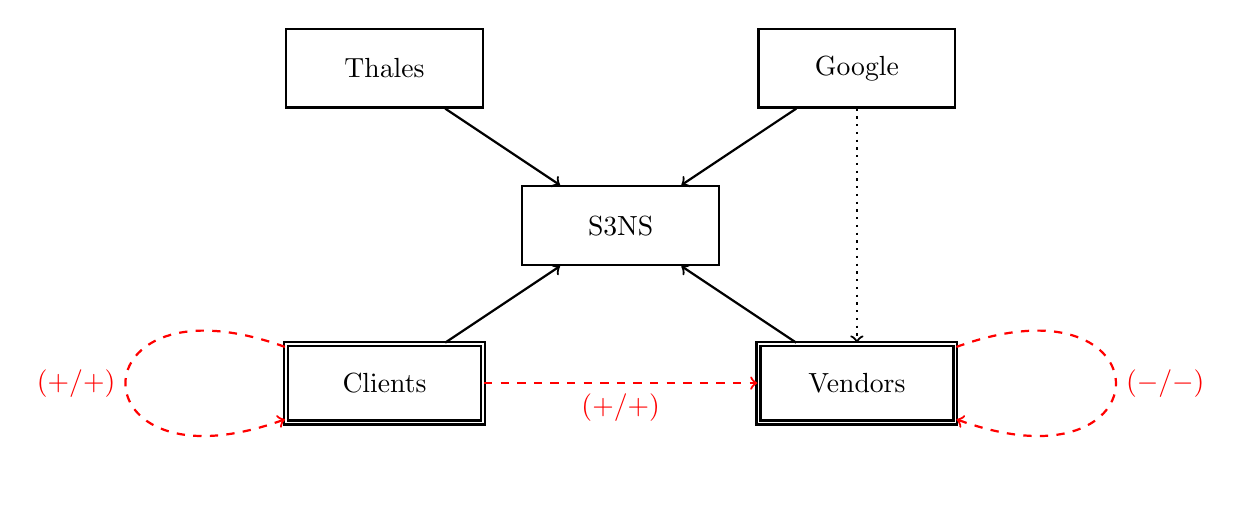
\begin{tikzpicture}[thick, ->]
  \node[draw, rectangle, minimum width=2.5cm, minimum height=1cm] (s3ns) at (0,0) {S3NS};
  \node[draw, rectangle, minimum width=2.5cm, minimum height=1cm] (thales) at (-3,2) {Thales};
  \node[draw, rectangle, minimum width=2.5cm, minimum height=1cm] (google) at (3,2) {Google};
  \node[draw, rectangle, double, minimum width=2.5cm, minimum height=1cm] (clients) at (-3,-2) {Clients};
  \node[draw, rectangle, double, minimum width=2.5cm, minimum height=1cm] (vendors) at (3,-2) {Vendors};

  \draw (thales) -- (s3ns);
  \draw (google) -- (s3ns);
  \draw (clients) -- (s3ns);
  \draw (vendors) -- (s3ns);
  \draw[dotted] (google) -- (vendors);
  \draw[red, dashed] (clients) -- (vendors) node[midway, below] {(+/+)};

  % Self-loops: weak same-side effects
  \draw[red, dashed] (clients) to[out=160, in=200, looseness=8] node[left] {(+/+)} (clients);
  \draw[red, dashed] (vendors) to[out=20, in=-20, looseness=8] node[right] {($-$/$-$)} (vendors);
\end{tikzpicture}
\caption{SRM of PREMI3NS}
\label{fig:srm}
\end{figure}

Money and control primarily meet in S3NS. The (+/+) cross-side effect between clients and vendors is the main network effect. There is only a weak (+/+) bandwagon effect among clients, and a ($-$/$-$) effect from competition among vendors. Much of what makes the platform attractive to vendors comes from Google through compatible skills, APIs and tools, and not from the alliance. Jointly, the BMC and the SRM show that the distribution of fixed costs and risks is carried by Thales, while Google owns the technology and earns from volume. 